\documentclass[tikz,border=8pt]{standalone}
\usetikzlibrary{arrows.meta,positioning,calc}
\makeatletter
\AtBeginDocument{\global\let\pgf@selectfontorig\relax}
\makeatother

\tikzset{
  nodebox/.style={draw=black, rounded corners=4pt, very thick, fill=gray!4,
    minimum width=10mm, minimum height=7mm, align=center, inner sep=2pt},
  initial/.style={-Latex, very thick},
  edge/.style={-Latex, thick, shorten >=1pt, shorten <=1pt},
  labelbox/.style={fill=white, inner sep=1.2pt, font=\scriptsize},
  aptxt/.style={font=\scriptsize, text=gray!65!black, anchor=north east},
}

\newcommand{\initarrow}[2]{\draw[initial] #1 -- (#2);}
\newcommand{\statelabel}[2]{\node[aptxt] at ($(#1.south east)+(0.02,-0.05)$) {#2};}

\begin{document}
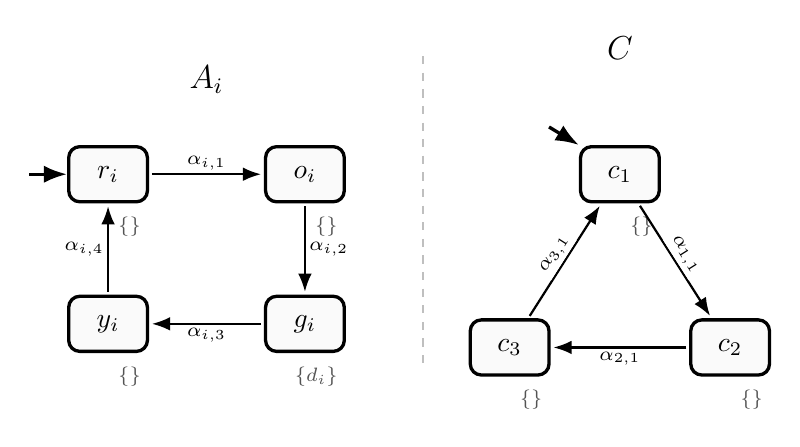
\begin{tikzpicture}[scale=1, transform shape]

  %% ---- A_i (left panel) ----
  \begin{scope}[shift={(0,0)}]
    \node[font=\bfseries\large] at (1.25, 1.2) {$A_i$};

    \node[nodebox] (r) at (0,    0  ) {$r_i$};
    \node[nodebox] (o) at (2.5,  0  ) {$o_i$};
    \node[nodebox] (g) at (2.5, -1.9) {$g_i$};
    \node[nodebox] (y) at (0,   -1.9) {$y_i$};

    \statelabel{r}{$\{\}$};
    \statelabel{o}{$\{\}$};
    \statelabel{g}{$\{d_i\}$};
    \statelabel{y}{$\{\}$};

    \initarrow{(-1.0, 0)}{r.west}

    \draw[edge] (r) -- node[labelbox, above] {$\alpha_{i,1}$} (o);
    \draw[edge] (o) -- node[labelbox, right] {$\alpha_{i,2}$} (g);
    \draw[edge] (g) -- node[labelbox, below] {$\alpha_{i,3}$} (y);
    \draw[edge] (y) -- node[labelbox, left]  {$\alpha_{i,4}$} (r);
  \end{scope}

  %% ---- Vertical divider ----
  \draw[dashed, gray!50, thick] (4.0, 1.5) -- (4.0, -2.4);

  %% ---- Controller C -- Neither variant (right panel) ----
  %% A_i center = y=-0.95; C triangle: nodes at y=1.4,-0.8,-0.8, init at y=2.0
  %% C center in scope ~ (2.0 + (-1.1))/2 = 0.45
  %% Shift C down by 0.95+0.45=1.40 to align centers
  \begin{scope}[shift={(6.5,-1.40)}]
    \node[font=\bfseries\large] at (0, 3.0) {$C$};

    \node[nodebox] (b1) at ( 0,    1.4) {$c_1$};
    \node[nodebox] (b2) at ( 1.4, -0.8) {$c_2$};
    \node[nodebox] (b3) at (-1.4, -0.8) {$c_3$};

    \statelabel{b1}{$\{\}$};
    \statelabel{b2}{$\{\}$};
    \statelabel{b3}{$\{\}$};

    \initarrow{(-0.9, 2.0)}{b1.north west}

    \draw[edge] (b1) -- node[labelbox, sloped, above] {$\alpha_{1,1}$} (b2);
    \draw[edge] (b2) -- node[labelbox, below]          {$\alpha_{2,1}$} (b3);
    \draw[edge] (b3) -- node[labelbox, sloped, above] {$\alpha_{3,1}$} (b1);
  \end{scope}

\end{tikzpicture}
\end{document}

    \statelabel{y}{$\{\}$};

    \initarrow{(-1.0, 0)}{r.west}

    \draw[edge] (r) -- node[labelbox, above] {$\alpha_{i,1}$} (o);
    \draw[edge] (o) -- node[labelbox, right] {$\alpha_{i,2}$} (g);
    \draw[edge] (g) -- node[labelbox, below] {$\alpha_{i,3}$} (y);
    \draw[edge] (y) -- node[labelbox, left]  {$\alpha_{i,4}$} (r);
  \end{scope}

  %% ---- Controller C -- Neither variant (right panel) ----
  %% A_i center ≈ y=-0.95; C triangle center ≈ y=0.3 before shift
  %% shift down by 1.25 to align centers
  \begin{scope}[shift={(6.5,-1.25)}]
    \node[font=\bfseries\large] at (0, 2.4) {$C$};

    \node[nodebox] (b1) at ( 0,    1.4) {$c_1$};
    \node[nodebox] (b2) at ( 1.4, -0.8) {$c_2$};
    \node[nodebox] (b3) at (-1.4, -0.8) {$c_3$};

    \statelabel{b1}{$\{\}$};
    \statelabel{b2}{$\{\}$};
    \statelabel{b3}{$\{\}$};

    \initarrow{(-0.9, 2.0)}{b1.north west}

    \draw[edge] (b1) -- node[labelbox, sloped, above] {$\alpha_{1,1}$} (b2);
    \draw[edge] (b2) -- node[labelbox, below]          {$\alpha_{2,1}$} (b3);
    \draw[edge] (b3) -- node[labelbox, sloped, above] {$\alpha_{3,1}$} (b1);
  \end{scope}

\end{tikzpicture}
\end{document}
